\documentclass{beamer}
\usepackage[utf8]{inputenc}
\usepackage{capt-of}
\usepackage[american]{babel}
\usepackage{csquotes}
\usepackage[style=ieee,backend=biber]{biblatex}


\usetheme{Madrid}
\usecolortheme{default}

\let\oldfootnoterule\footnoterule
\def\footnoterule{\only<2->\oldfootnoterule}

\DeclareLanguageMapping{american}{american-apa}
\addbibresource{biblio.bib}
\setbeamertemplate{bibliography item}{\insertbiblabel}

%------------------------------------------------------------
%This block of code defines the information to appear in the
%Title page
\title[Complex Exponentials] %optional
{Complex Exponentials}

\subtitle{A can of worms we shall open!}

\author[R. Mok] % (optional)
{R.~Mok BSc(AdvMath), MTeach, GradCertDS}

\date[August 2021] % (optional)
{AISNSW Mathematics Heads of Department Conference, August 2021}

% \logo{\includegraphics[height=1cm]{overleaf-logo}}

%End of title page configuration block
%------------------------------------------------------------



%------------------------------------------------------------
%The next block of commands puts the table of contents at the
%beginning of each section and highlights the current section:

\AtBeginSection[]
{
  \begin{frame}
    \frametitle{Table of Contents}
    \tableofcontents[currentsection]
  \end{frame}
}
%------------------------------------------------------------


\begin{document}

%The next statement creates the title page.
\frame{\titlepage}


%---------------------------------------------------------
%This block of code is for the table of contents after
%the title page
\begin{frame}
\frametitle{Table of Contents}
\tableofcontents
\end{frame}
%---------------------------------------------------------


\section{Opening Question}

%---------------------------------------------------------
%Changing visivility of the text
\begin{frame}
\frametitle{Opening Question}
Here's a few questions to warm you up for the session to see if you're awake!

\begin{enumerate}
  \item Solve for $x \in \mathbb{N}: x^2 = 4$\\
    A) $x = 2\quad$ B) $x = 4^{\frac{1}{2}}\quad$ C) $x = \pm 2\quad$ D) $x= \sqrt{4}$
  \item Solve for $x \in \mathbb{R}: x^2 = 4$\\
    A) $x = 2\quad$ B) $x = 4^{\frac{1}{2}}\quad$ C) $x = \pm 2\quad$ D) $x= \sqrt{4}$
  \item Solve for $x \in \mathbb{C}: x^2 = 4$\\
    A) $x = 2\quad$ B) $x = 4^{\frac{1}{2}}\quad$ C) $x = \pm 2\quad$ D) $x= \sqrt{4}$
\end{enumerate}
\pause
Answers:
\begin{enumerate}
  \item A, B and D
  \item C
  \item \alert{B and C}
\end{enumerate}
\end{frame}

%---------------------------------------------------------

\section{Revisiting De Moivre's Theorem}

%---------------------------------------------------------
%Highlighting text
\begin{frame}
\frametitle{De Moivre's Theorem}
\begin{block}{De Moivre's Theorem (DMT)\parencite{syllabus}}
  \begin{itemize}
    \item[]<3-> For all \alert{integers $n$}
    \item[]<1-> \[[r(\cos\theta + i \sin\theta)]^n = r^n(\cos(n\theta) + i\sin(n\theta))\]
    \item[]<4-> This is to ensure the exponential of a complex number yields one value for all arguments of that complex number.
  \end{itemize}
  \end{block}
  \pause
  \begin{block}{Pythagoras' Theorem}
  \begin{itemize}
    \item[]<3-> A triangle with side lengths $a,b,c$ is right angled if and only if
    \item[]<1-> \[c^2 = a^2 + b^2\]
  \end{itemize}
\end{block}
\pause
DESMOS Interactive: \url{https://www.desmos.com/calculator/szywgvtxm8}
\end{frame}

\begin{frame}
\frametitle{Extending De Moivre's Theorem to Rational Exponents}
If we want to extend DMT to rational exponents, this happens:
\begin{example}
  \begin{align*}
    1 & = (\cos 0 + i \sin 0) \mbox{ or } (\cos 2\pi + i\sin 2 \pi)\\
    1^\frac{1}{2} & = (\cos 0 + i \sin 0)^\frac{1}{2} \mbox{ or }(\cos 2\pi + i\sin 2 \pi)^\frac{1}{2}\\
                  & = \cos 0 + i \sin 0 \mbox{ or } \cos \pi + i \sin \pi\\
                  & = 1 \mbox{ or } -1
  \end{align*}
\end{example}
\pause
Exponentials of complex numbers are \alert{multi-valued} functions\footnote<2->{HSC uses the terminology `one-to-many' relation.}.
\end{frame}

\begin{frame}
  \frametitle{Roots of Unity}
  This process is essentially how Roots of Unity are found:
  \begin{example}
    \begin{align*}
      z^n & = 1\\
          & = (\cos (2k\pi) + i\sin (2k\pi)) \mbox{ for } k \in \mathbb{Z}\\
      z & = \cos\left(\frac{2k\pi}{n}\right) + i\sin \left(\frac{2k\pi}{n}\right) \mbox{by the \alert{extended} DMT}
    \end{align*}
  \end{example}
\end{frame}

\begin{frame}
  \frametitle{Back to the opening question}
  \begin{block}{Opening Question}
Solve for $x \in \mathbb{C}: x^2 = 4$\\
A) $x = 2\quad$ \alert{B) $x = 4^{\frac{1}{2}}\quad$ C) $x = \pm 2\quad$} D) $x= \sqrt{4}$
\end{block}
\pause
Note: $\sqrt{4} = 2$, $4^\frac{1}{2} = \pm 2$

\pause
$\sqrt{\cdot}: \mathbb{C} \rightarrow \mathbb{C}$ is single-valued and is restricted to the principal argument. However, the exponential is multi-valued.

\pause
What even is an exponential then? More on that later...
\end{frame}

\begin{frame}
  \frametitle{Complex Exponentials with Irrationals}
  \begin{itemize}
    \item<1-> Rational exponents $m/n$ divide the revolutions of arguments nicely such that their results repeat themselves with periodicity (at most) $n$.
    \item<2-> Irrational exponents do not divide the revolutions nicely and hence have infinite values.
  \end{itemize}
  \pause\pause
  \begin{center}
  \begin{minipage}{0.8\textwidth}
    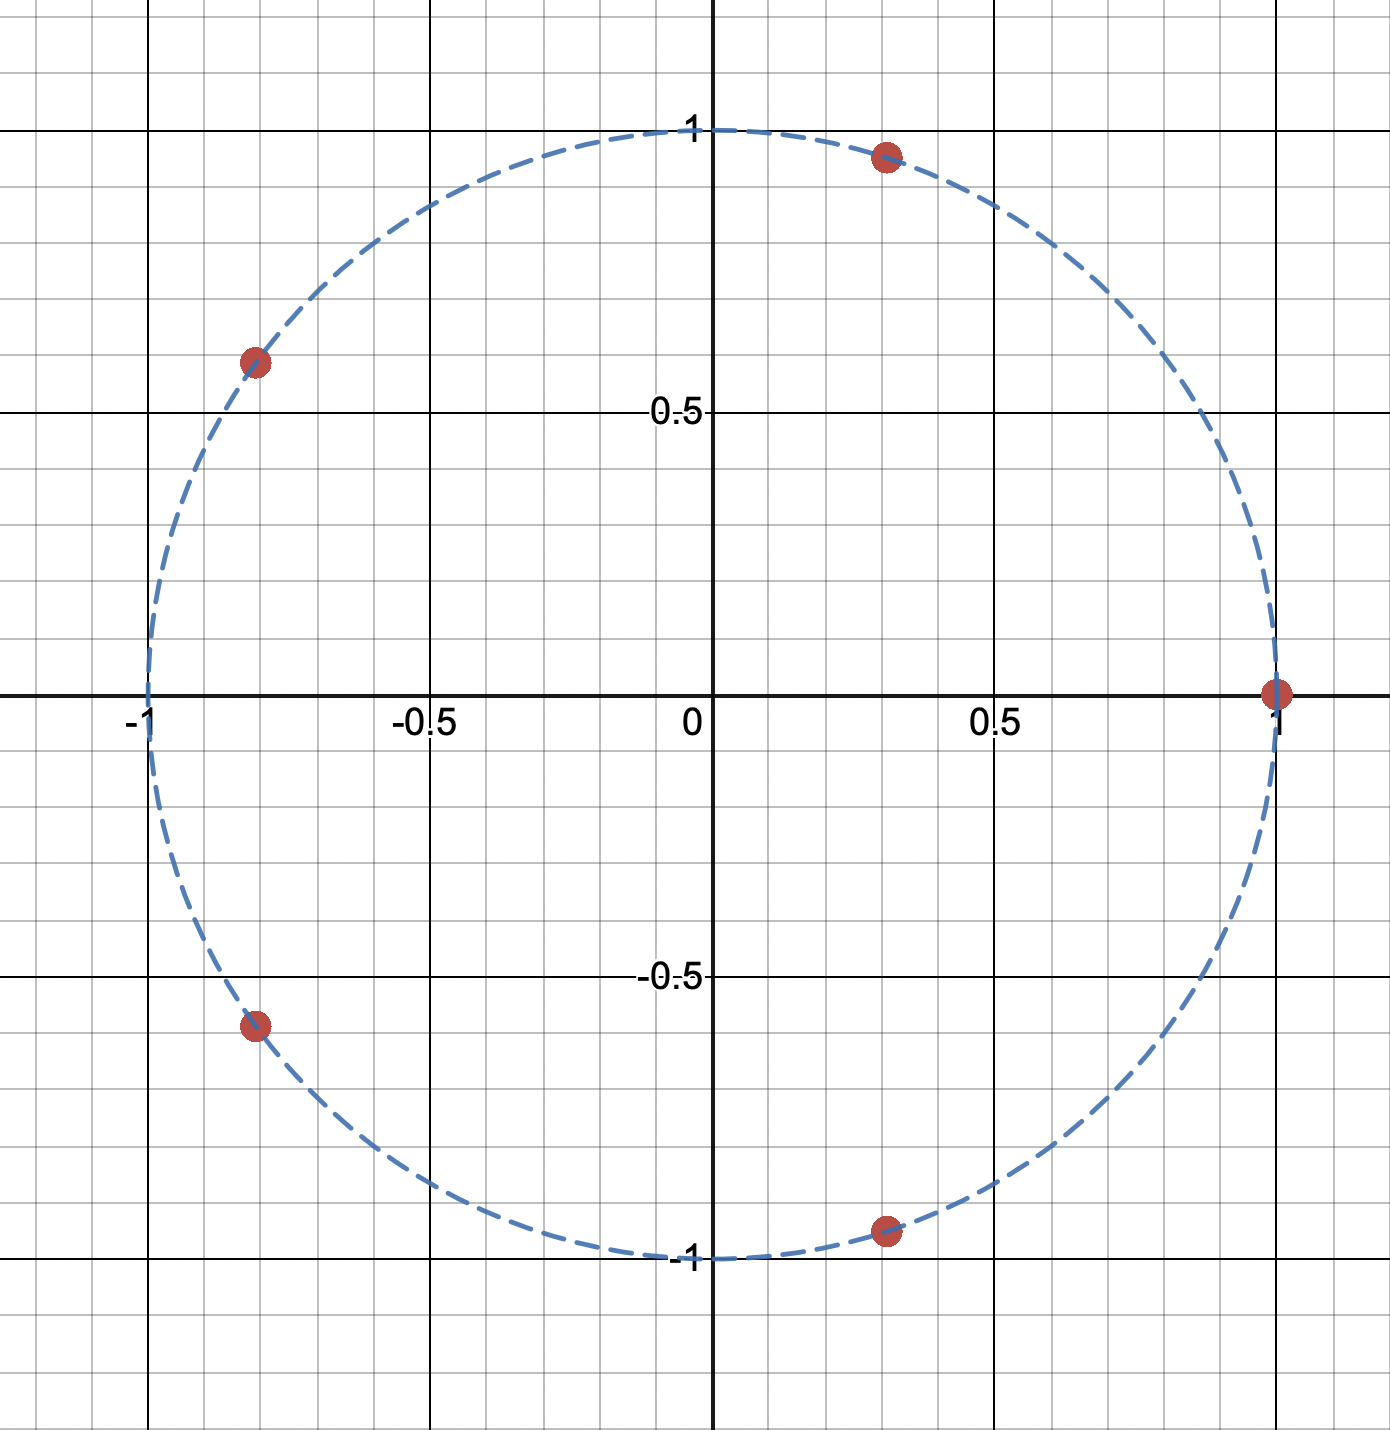
\includegraphics[width=0.45\textwidth]{fifth_roots.png}
    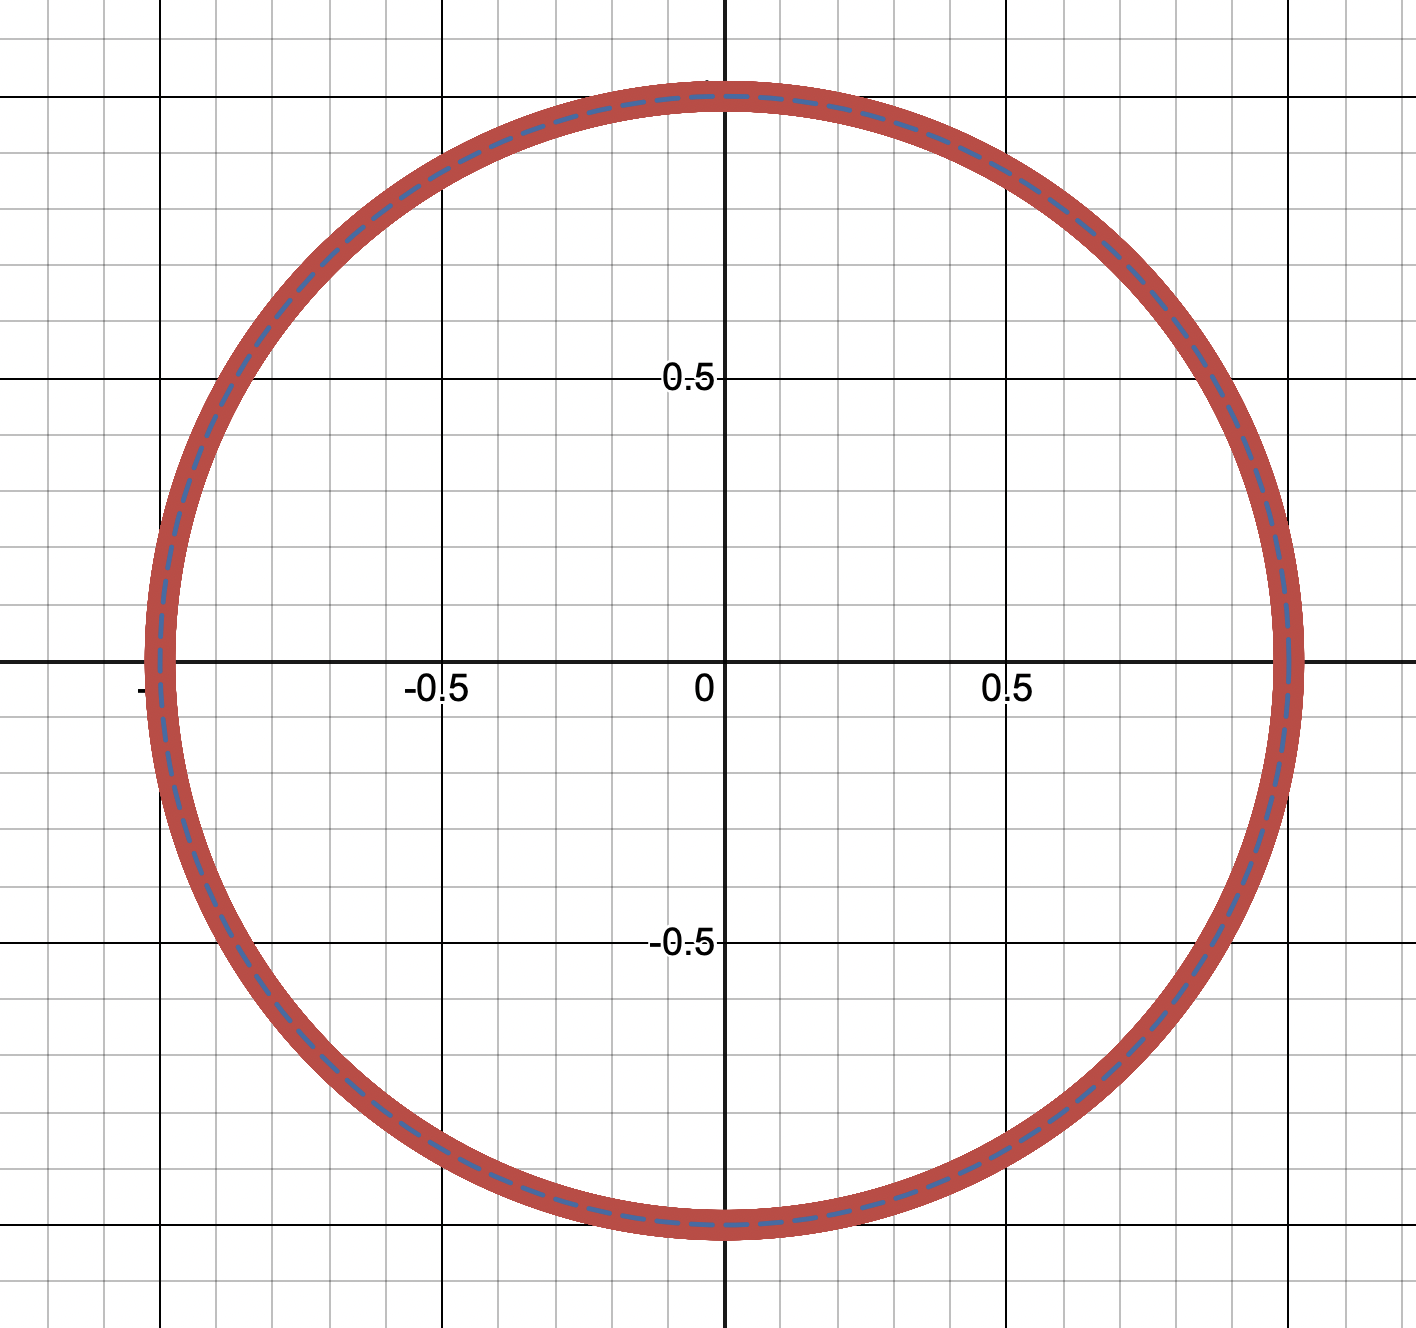
\includegraphics[width=0.45\textwidth]{irrational_roots.png}
    \captionof{figure}{$1^\frac{1}{5}$ vs. irrational exponents such as $1^\pi$, $(-1)^{\sqrt{2}}$, etc}
  \end{minipage}
  \end{center}
\end{frame}

\begin{frame}
  \frametitle{Quick Recap}
  \begin{itemize}
    \item<1-> De Moivre's Theorem (DMT) for integer exponents yields single values.
    \item<2-> Extending DMT to rational exponents $m/n$ yields (at most) $n$ values.
    \item<3-> Extending DMT to irrational exponents yields infinite values.
    \item<4-> What's next? Complex exponents.
  \end{itemize}
\end{frame}

%---------------------------------------------------------

\section{Euler's Formula}

%---------------------------------------------------------

\begin{frame}
  \frametitle{Euler's Formula}
  HSC Dotpoint MEX-N1.3 introduces Euler's Formula \parencite{syllabus} which was not in the old syllabus:
\begin{block}{Euler's Formula}
  \[ e^{ix} = \cos x + i \sin x \mbox{ for real } x\]
\end{block}
\pause
This opens up new avenues of discussion that were previously not possible in the old syllabus...

\pause
... such as:
\begin{block}{De Moivre's Theorem Restated}
  \[(e^{ix})^n = e^{inx}\]
  with the same discussions about $n$ as in the previous section.
\end{block}
\end{frame}

\begin{frame}
  \frametitle{Complex Logarithms}
  Euler's Formula opens up discussion about:
  \begin{align*}
    z &= |z|e^{i\arg z}\\
    \log z & = \log ( |z| e^{i\arg z} )
  \end{align*}
  \pause
  Does such a function $\log: \mathbb{C}\backslash\{0\} \rightarrow \mathbb{C}$ that is the inverse of complex exponentiation exist? Yes it does - proof beyond the time we have now.
  \pause
  \begin{block}{Complex Logarithm \parencite[p.~23]{apostol}}
    If $z$ is a complex number $\not = 0$, then there exist complex numbers $\omega$ such that $e^\omega = z$ where $\omega$ is in the form $\log_e|z| + i\mbox{Arg}z + 2n\pi i$ where $n\in\mathbb{Z}$.
  \end{block}
\end{frame}

\begin{frame}
  \frametitle{Complex Exponential Equations}
  \begin{example}
    Solve for $z \in \mathbb{C}: e^z = 1$.
    \pause
    \begin{align*}
      z & = \log(1)\\
        & = \log_e|1| + i\arg(1)\\
        & = 0 + i\arg(1)\\
        & = i2k\pi \mbox{ for } k \in \mathbb{Z}
    \end{align*}
  \end{example}
  \pause
  If we test any of these solutions such as $z_1 = i2\pi$:
  \begin{align*}
    e^{z_1} & = e^{i2\pi} = 1
  \end{align*}
  Hence, $i2\pi$ is indeed a solution to $e^z = 1$.
\end{frame}

\begin{frame}
  \frametitle{Complex Trigonometric Equations}
  It can be shown using Euler's Formula that:
  \begin{block}{Trigonometric Functions}
    \[\cos z = \frac{e^{iz} + e^{-iz}}{2}\]
    \[\sin z = \frac{e^{iz} - e^{-iz}}{2i}\]
  \end{block}
\end{frame}
\begin{frame}
  \frametitle{Complex Trigonometric Equations}
  \begin{example}
  Solve for $z \in \mathbb{C}: \sin z = 2$
  \pause
  \begin{align*}
    \frac{e^{iz} + e^{-iz}}{2} & = 2\\
    e^{iz} + e^{-iz} & = 4\\
    e^{2iz} - 4e^{iz} + 1 & = 0\\
    e^{iz} & = \frac{4 \pm \sqrt{4^2 - 4(1)(1)}}{2} = 2 \pm \sqrt{3}\\
    iz & = \log_e(2 \pm \sqrt{3}) + i2k\pi \mbox{ for } k \in \mathbb{Z}\\
    z & = \frac{1}{i}\log_e(2 \pm \sqrt{3}) + 2k\pi
  \end{align*}
  \end{example}
\end{frame}

\begin{frame}
  \frametitle{Complex Exponents}
  \begin{example}
    Evaluate $i^i$.
    \pause
    \begin{align*}
      i^i & = e^{\log i^i}\\
          & = e^{i \log i}\\
          & = e^{i (\log_e|i| + i\arg i)}\\
          & = e^{i^2 \arg i}\\
          & = e^{-1(\frac{\pi}{2} + 2k\pi)} \mbox{ for } k \in \mathbb{Z}\\
          & = \ldots, 111.3177784899\ldots, 0.2078795764\ldots, 0.0003882032039\ldots, \ldots
    \end{align*}
  \end{example}
  % \pause
  % In the same way, we can show $1^i = e^{-2k\pi}$ for $k \in \mathbb{Z}$.
\end{frame}

\begin{frame}
  \frametitle{More examples}
  \begin{example}
    \begin{itemize}
      \item Evaluate $1^i$.
      \item Evaluate $(-1)^{\sqrt{2}}$.
    \end{itemize}
  \end{example}
  \pause
  Answers:
  \[1^i = e^{-2k\pi} \mbox{ for } k \in \mathbb{Z}\]
  \[(-1)^{\sqrt{2}} = e^{\sqrt{2}i\pi(2k+1)} \mbox{ for } k \in \mathbb{Z}\]
\end{frame}

%---------------------------------------------------------

\section{What is an exponential?}

%---------------------------------------------------------

\begin{frame}
  \frametitle{A progressive relearning at each stage}
  \begin{itemize}
    \item<1->Stage 4: A power is how many times that base multiplies itself.\\
      \[ 2^3 = 2\times 2 \times 2 = 8\]
      \pause
      Problem: How can $2^\frac{-1}{2}$ mean $\underbrace{2 \times \ldots \times 2}_{\frac{-1}{2} times}$?

    \item<3->Stage 5: Extend the concept of exponentials with index laws that fixes this problem.
    \item<4->Stage 6: The number $e$ is introduced in the topic of calculus. Jacob Bernoulli derived this value in 1683 when considering the compound interest problem of compounding a principal amount of \$1 at an ever increasing compounding period over a year. He arrived at the discovery:
      \[ e = \lim_{n\rightarrow \infty}\left(1 + \frac{1}{n}\right)^n \]
  \end{itemize}
\end{frame}

\begin{frame}
  \frametitle{Exponential Function}
  \begin{block}{$e$}
    \[ e = \lim_{n\rightarrow \infty}\left(1 + \frac{1}{n}\right)^n \]
    if and only if
    \[ e = \sum_{k=0}^\infty \frac{1}{k!}\]
  \end{block}
  The proof uses concepts in Binomial Theorem and Analysis \parencite[pp.~64-65]{rudin}.

  It can also be shown (using similar methods as in the proof) that:
  \begin{block}{Exponential Function \parencite[p.~174]{rudin}}
    \[\exp(x) = \sum_{k=0}^\infty \frac{x^k}{k!} = \lim_{n\rightarrow\infty}\left(1 + \frac{x}{n}\right)^n \]
  \end{block}
\end{frame}

\begin{frame}
  \frametitle{What is an exponential?}
  \begin{block}{So what is an exponential? \parencite[p.~46]{ahlfors}}
    $a^b$ is equivalent to $\exp(b \log a)$.

    If $a$ is restricted to positive numbers, $\log a$ shall be real and $a^b$ has a single value.

    Otherwise, $\log a$ is the complex logarithm and $a^b$ has in general infinitely many values.
  \end{block}
\end{frame}

\begin{frame}
  \begin{block}{Plots of increasing $n$ for $(1 + \frac{x}{n})^n$}
  DESMOS Interactive: \url{https://www.desmos.com/calculator/p4rzq24eck}\\
  Plots of $(1+\frac{x}{n})^n$ for $x = 1$ or $x=i\pi$ and differing values of $n$ are shown below:
  \end{block}
  \begin{minipage}{\textwidth}
    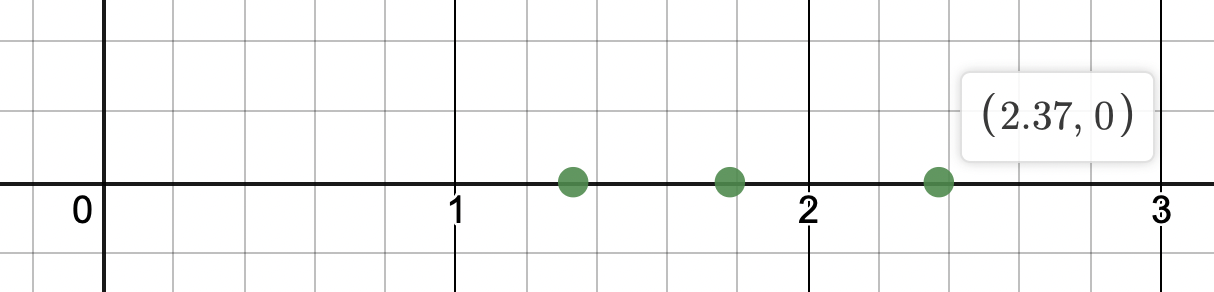
\includegraphics[width=0.47\textwidth]{real_exp_3.png}
    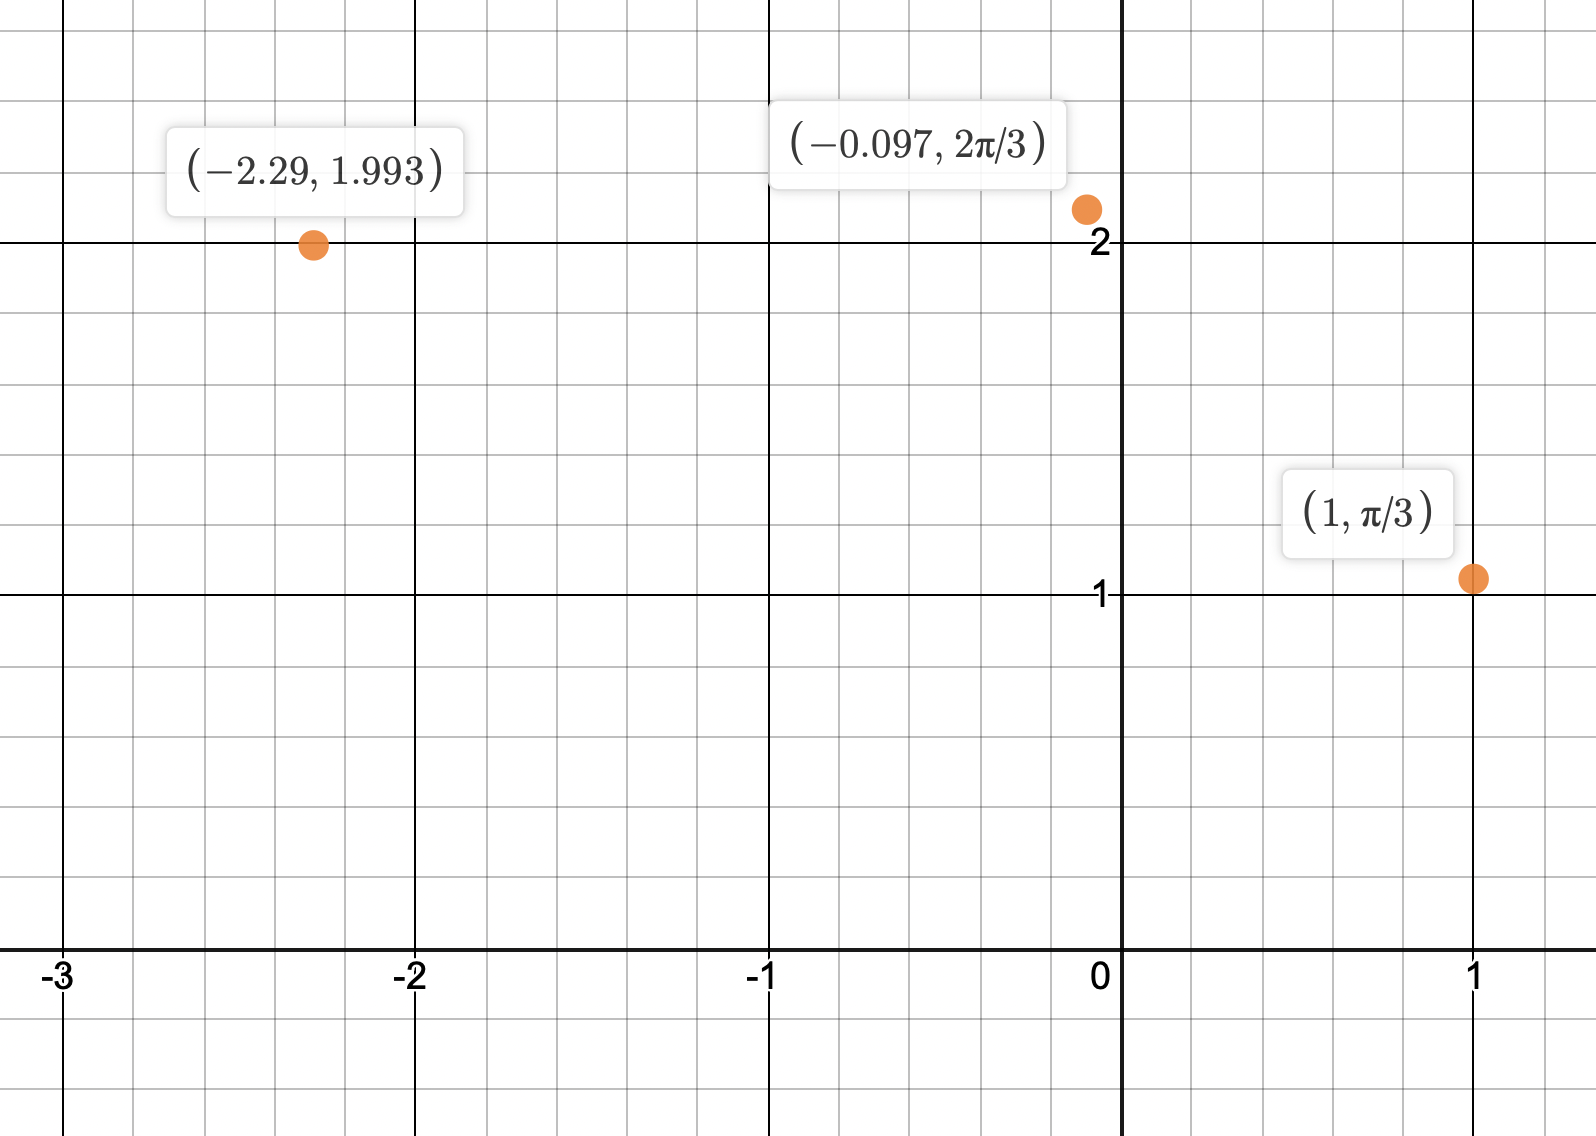
\includegraphics[width=0.47\textwidth]{complex_exp_3.png}
    \captionof{figure}{$(1+\frac{x}{3})^n$ for $n=1,2,3$}
  \end{minipage}
\end{frame}

\begin{frame}
  \begin{block}{Plots of increasing $n$ for $(1 + \frac{x}{n})^n$}
  DESMOS Interactive: \url{https://www.desmos.com/calculator/p4rzq24eck}\\
  Plots of $(1+\frac{x}{n})^n$ for $x = 1$ or $x=i\pi$ and differing values of $n$ are shown below:
  \end{block}
  \begin{minipage}{\textwidth}
    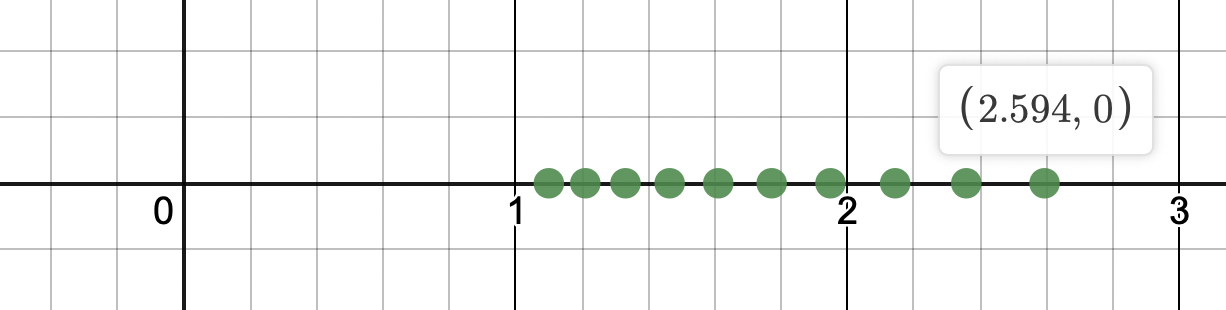
\includegraphics[width=0.47\textwidth]{real_exp_10.png}
    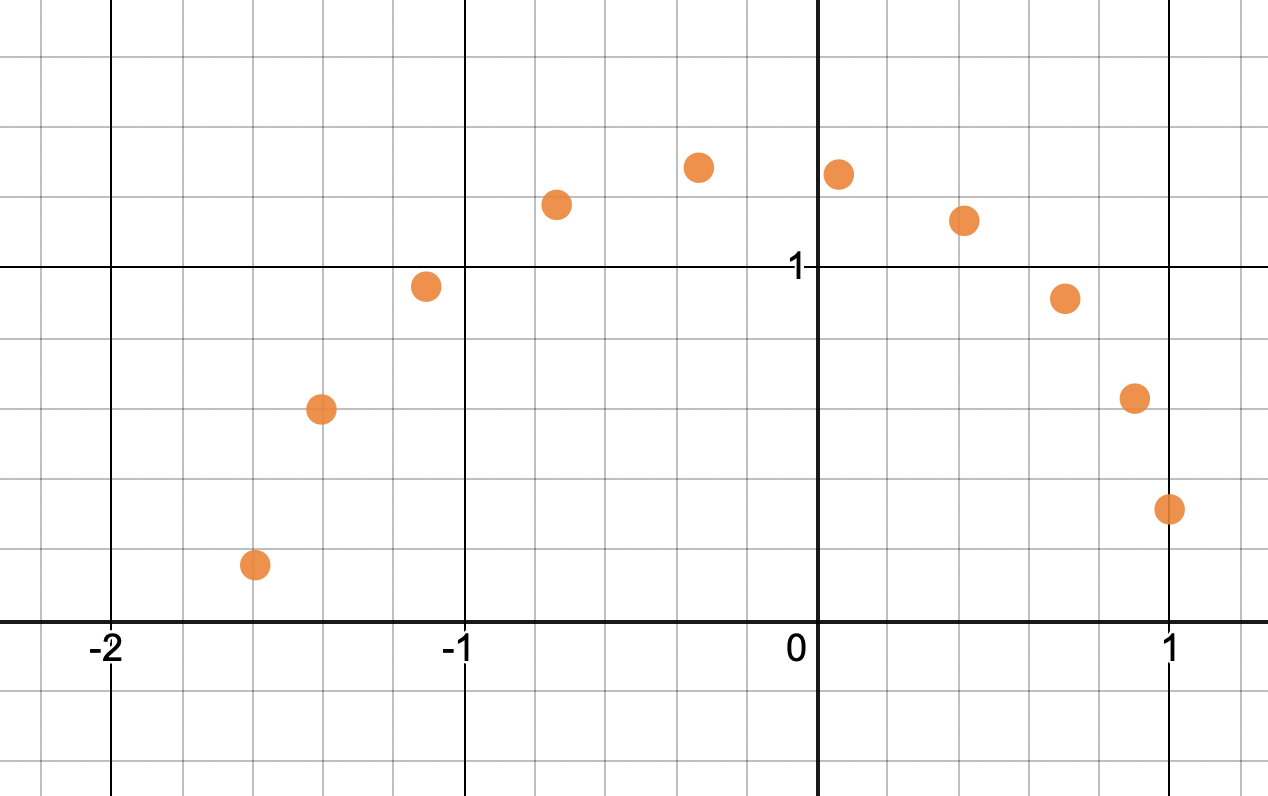
\includegraphics[width=0.47\textwidth]{complex_exp_10.png}
    \captionof{figure}{$(1+\frac{x}{10})^n$ for $n=1,2,\ldots,10$}
  \end{minipage}
\end{frame}

\begin{frame}
  \begin{block}{Plots of increasing $n$ for $(1 + \frac{x}{n})^n$}
  DESMOS Interactive: \url{https://www.desmos.com/calculator/p4rzq24eck}\\
  Plots of $(1+\frac{x}{n})^n$ for $x = 1$ or $x=i\pi$ and differing values of $n$ are shown below:
  \end{block}
  \begin{minipage}{\textwidth}
    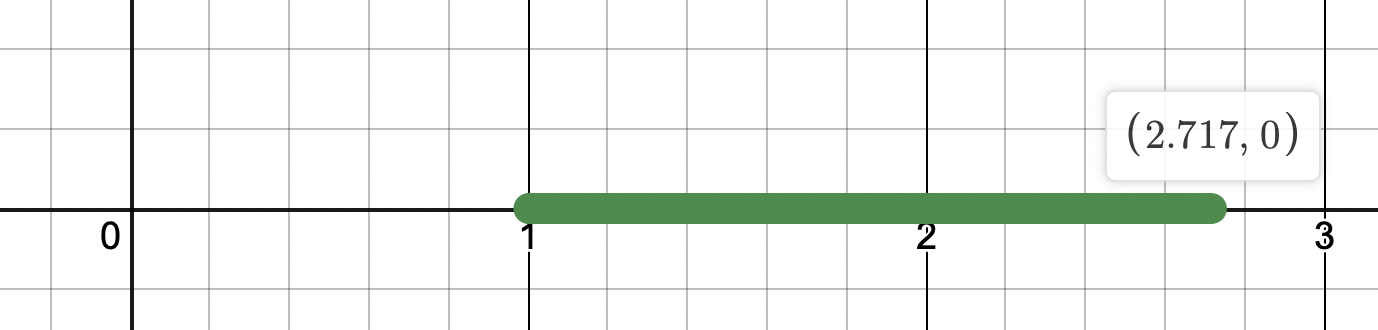
\includegraphics[width=0.47\textwidth]{real_exp_1000.png}
    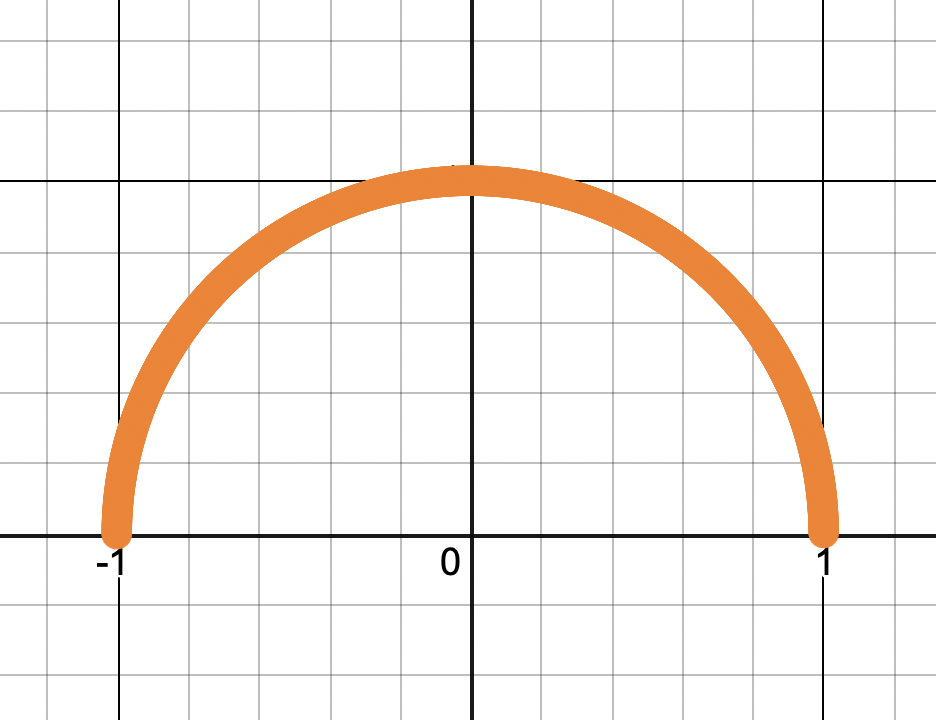
\includegraphics[width=0.47\textwidth]{complex_exp_1000.png}
    \captionof{figure}{$(1+\frac{x}{1000})^n$ for $n=1,2,\ldots,1000$}
  \end{minipage}
\end{frame}

\section{Bibliography}
\begin{frame}
  \frametitle{Bibliography}
  \printbibliography

  Source files and PDF for this presentation can be found on:
  \url{https://github.com/moksifu/complex_exponentials}
  under the MIT Licence.
\end{frame}


%---------------------------------------------------------


\end{document}
